%%\section*{BGRa model}

 The BGRa stationary creep model defines
 the uniaxial creep strain increment as
\begin{equation}
\Delta\strain^c=Ae^{-Q/R_uT}\left(\dfrac{\stress}{\stress_f}\right)^m \Delta t
 \label{eq:cstrain}
\end{equation}
where $A$, $m$ and $Q$ are parameters determined by experiments, $Q$ is called activation energy,
 $R_u=8.314472 \mbox{J/(Kmol)}$ is the universal gas constant and $\stress_f=1\mbox{MPa}$, a stress scaling factor.
\subsection*{Creep potential}
Assume there is a creep potential $g$ and the creep induced strain rate is given by the flow rule
\begin{gather}
\dot \Strain^c (\stress)= \pD{g^c}{\Stress}
\label{eq:cflowrule}
\end{gather}
Since the first stress invariant $\stress$ is given by $\stress={\color{black}\sqrt{{\frac{3}{2}}}}\norm{\devStrs}$ with $\devStrs = \Stress-\frac{1}{3}\stress\I$, the deviatoric stress,
the creep strain rate is then expressed as
\begin{gather}
\dot \Strain^c (\stress)= \pD{g^c}{\stress}\pD{\stress}{\Stress}=\pD{g^c}{\stress}\dfrac{\devStrs}{\stress}
\label{eq:cflowrule2}
\end{gather}
Expression (\ref{eq:cflowrule2}) must be valid for the problems with different dimension. Applying (\ref{eq:cflowrule2})
to one dimensional creep strain expression (\ref{eq:cstrain}), we have
\begin{gather}
\dot \strain^c = \pD{g^c}{\stress}{\color{black}\dfrac{2}{3}}=Ae^{-Q/R_uT}\left(\dfrac{\stress}{\stress_f}\right)^m
\label{eq:cflowrule3}
\end{gather}
Therefore, the creep strain rate for multi-dimensional problems can be derived as
\begin{gather}
 \dot \Strain^c (\stress)={\color{black}\dfrac{3}{2}}Ae^{-Q/R_uT}\left(\dfrac{\stress}{\stress_f}\right)^m\dfrac{\devStrs}{\stress}
\label{eq:crpstrain}
\end{gather}
\subsection*{Example}
We verify the scheme by a one dimensional extension with constant pressure of $\stress_0=\mbox{5MPa}$. The values of the parameters are given as
$A=0.18 \mbox{d}^{-1}$, $m=5$, $Q=54\mbox{kJ/mol}$, $E=25000\mbox{MPa}$, and the temperature is constant everywhere of $100^{\circ}\mbox{C}$.
The analytical solution of the strain is given straightforward as
\begin{gather}
\strain=-\dfrac{\stress_0}{E}-Ae^{-Q/RT}\stress_0^n t
\label{eq:cflowrule}
\end{gather}
The comparison of the results obtained by the present multidimensional scheme with the analytical solution is shown in Fig. \ref{fig:cmp}

\begin{figure}[H]
  \centering
  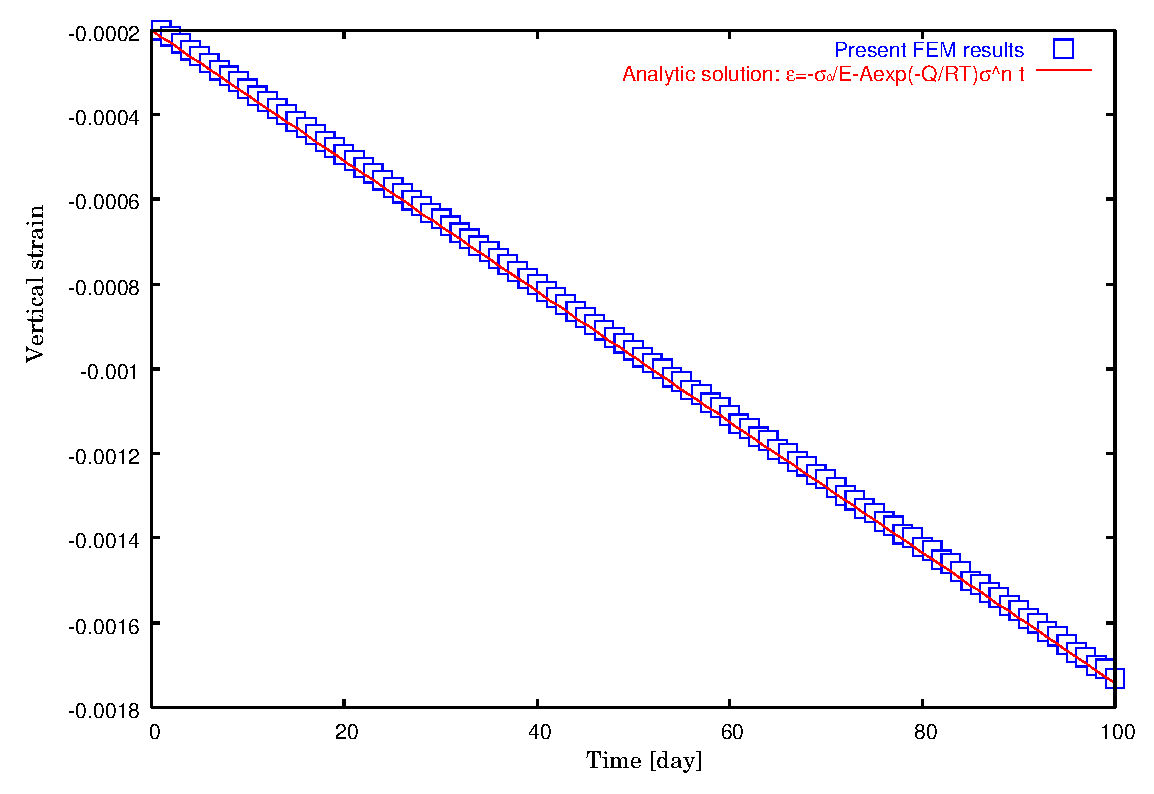
\includegraphics[scale=0.5]{M/crp/bgra0.eps}
  \caption{Comparision}
  \label{fig:cmp}
\end{figure}
